\documentclass[a4paper,11pt]{article} 

% ===== Algunos paquetes a ser usados =====

% para poder escribir con tildes   
\usepackage[T1]{fontenc}           
\usepackage[utf8]{inputenc}        
\usepackage[spanish]{babel}        

\spanishdecimal{.}        
\usepackage{times}        

\usepackage{animate}        

% fuentes para escribir símbolos 
\usepackage{amsfonts}            
\usepackage{amssymb}             
\usepackage{amsthm}              
\usepackage{mathrsfs}            
\usepackage[centertags]{amsmath}    

% inclusión de graficos    
\usepackage{graphicx}      

% símbolo de grados    
\newcommand{\grad}{\hspace{-2.5mm}$\,\phantom{a}^{\circ}\,$}        

% ==================================== 

% ========= Referencias ==========           
\usepackage{hyperref}                        
% ================================           

% ========= Color ==========           
\usepackage[usenames,dvipsnames]{color}                         
% ================================           

% ===== Ajuste layout pagina =====           
\textheight=23cm                            
\textwidth=18cm                              
\topmargin=-1cm                              
\oddsidemargin=-1cm                           
\parindent=0mm                               
\usepackage{fancyhdr}                        
% ================================           

% ========= Comandos ==========           
\newcommand{\ds}{\displaystyle}         
\def\x{{\bf x}}                         
% ================================           

% ========= Tablas y otros ==========           
%\usepackage[table]{xcolor} % Sirve para poner letras con colores y colorear tablas            
\addto\captionsspanish{ \renewcommand{\tablename}{Tabla}} %Uso tabla en vez de cuadro        
\addto\captionsspanish{ \renewcommand{\appendixname}{Apéndice}}                               
%\addto\captionsspanish{ \renewcommand{\appendixpagename}{Apéndice}}                         
%\addto\captionsspanish{ \renewcommand{\appendixtocname}{Apéndice}}                          
%\addto\captionsspanish{ \renewcommand{\lstlistingname}{Rutina}}                             
\usepackage{array}                                                                               
\newcolumntype{C}[1]{>{\centering\let\newline\\\arraybackslash\hspace{0pt}}m{#1}}         
\newcolumntype{L}[1]{>{\raggedright\let\newline\\\arraybackslash\hspace{0pt}}m{#1}}       
\newcolumntype{R}[1]{>{\raggedleft\let\newline\\\arraybackslash\hspace{0pt}}m{#1}}        
\usepackage{booktabs}                                                                            
\usepackage{longtable}                                                                            
% ================================           

\newpage  

\begin{document}      

% == Encabezado y pie de pagina ==           
\pagestyle{fancy}                            
\cfoot{}                                     
\lhead{Project name}                  
\lfoot{\footnotesize Complete Small Deformations and Displacements Output}      
\rfoot{Page \thepage}                        
% ================================           

% ======== Texto ==========  

\begin{minipage}[t]{1\textwidth}      
\vspace{0.5mm}      
\noindent      
Curso de Elasticidad 2014 \\     
Ingeniería Civil - Plan 97 \\      
Materia: Resistencia de Materiales      

\begin{center}      
\textbf{\Large{ Input file:}}\Large{ \verb+Prueba.txt+}  \\      
\large{Project name \\}       
\today\\      
IETFEM v2.11      
\vspace{-2.9cm}      
\end{center}      
\end{minipage}      
\hspace{-2cm}      
\begin{minipage}[t]{.1\textwidth}      
\vspace{0.0mm}      

\includegraphics[width=.95\textwidth]{../../../../../../sources/Figs/logo_udelar}      
\end{minipage}      

\vspace{1cm}       

\hspace{1.5cm}       
\begin{center}       
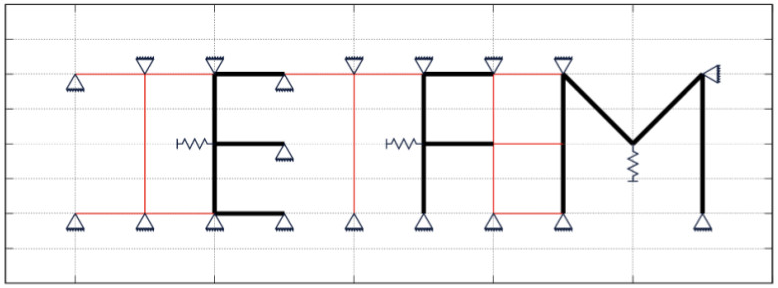
\includegraphics[width=.7\textwidth]{../../../../../../sources/Figs/logo_ietfem}      
\end{center}       
\begin{center}       
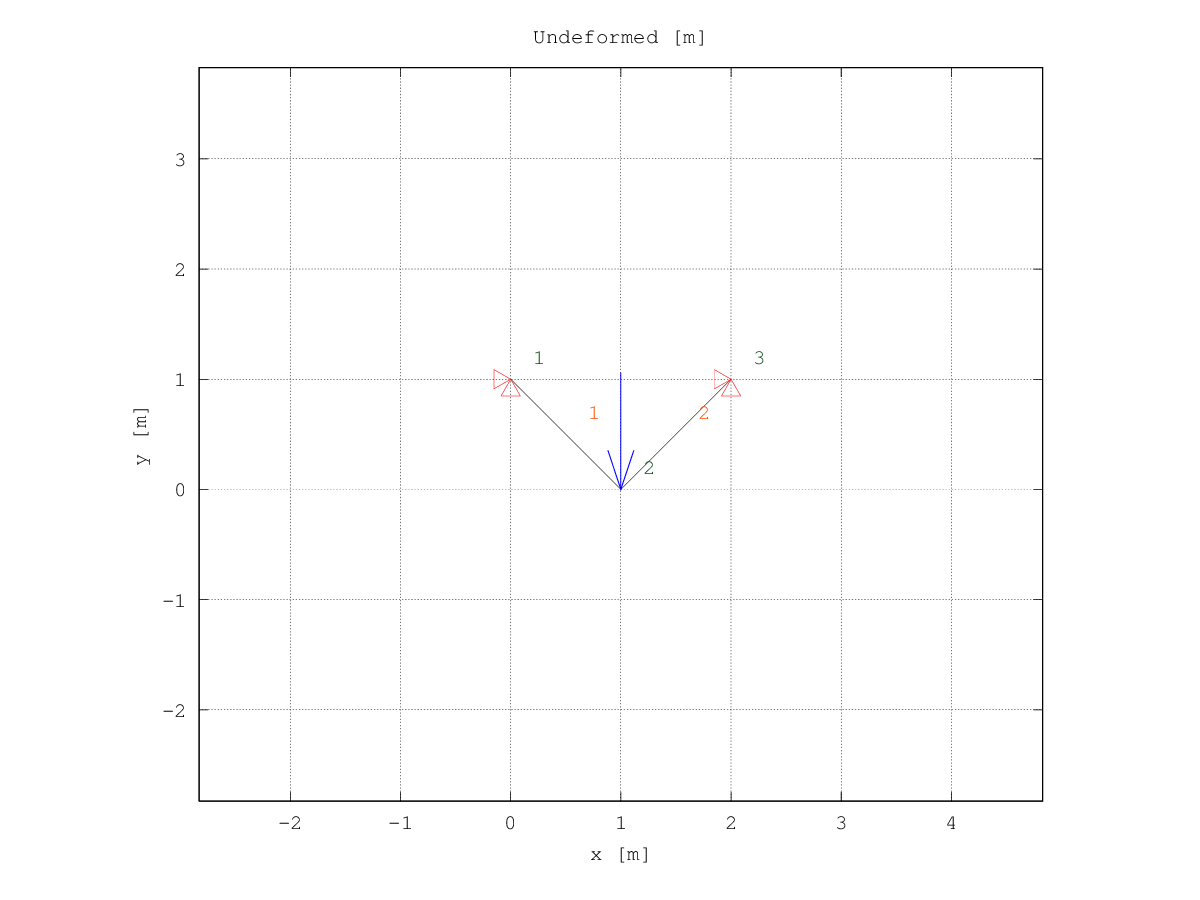
\includegraphics[width=.95\textwidth]{../../Prueba_undeformed.png}   
   \end{center}       

\newpage 

================== Complete Output IETFEM v2.11 ===========================\\
================== Linear elasticity solution ===========================
% hace índice        
\tableofcontents     

\newpage     

\section{General input}

Inputfile: \verb|../../input/2D/Truss_2D_sd/Prueba.txt|  ... \\

Solve time: $ 5.811$ seconds \\

Problem type: Truss 2D small deformations and displacements\\ 

Length magnitude: m \\

Force magnitude: kN \\

Number of degrees of freedom per node: 2 \\

Number of nodes per element: 2 \\

Number of materials: 1 \\

Number of sections: 2 \\

Number of nodes: 3 \\

Number of elements: 2 \\

Scales factors: 
\begin{itemize} 
\item  SD\_Deformed: 1 
\item  Supports: 0 
\item  Areas: 1 
\item  Forces: 2 
\item  Frame: 2 
\item  Numbers: 1 
\end{itemize} 
\newpage       

\section{Nodes cordinates} 

\begin{center}                                   
\begin{longtable}{|R{1.5cm}|R{2.4cm}|R{2.4cm}|}
\toprule[0.8mm]                                  
\multicolumn{3}{|c|}{Coordinates (m)   }  \\  
\midrule[0.5mm]                                  
Node & $X$ & $Y$          \\               
\midrule[0.5mm]                                  
\endfirsthead                                    
\toprule[0.8mm]                                  
\multicolumn{3}{|c|}{Coordinates (m)   }  \\  
\midrule[0.5mm]                                  
Node & $X$ & $Y$          \\               
\midrule[0.5mm]                                  
\endhead                                         
\hline                                           
\multicolumn{3}{r}{Next page...}                 
\endfoot                                         
\endlastfoot                                     
    1 & 0  &   1.00 \\ 
    2 &   1.00  & 0 \\
    3 &   2.00  &   1.00 \\ 
\bottomrule[0.8mm]                               
\caption{Nodes Coordinates}             
\end{longtable}                                  
\end{center}                                     

\newpage       

\section{Element's conectivity} 

Start: Start node - End: End node.
\begin{center}                                   
\begin{longtable}{|R{1.5cm}|R{1.5cm}|R{1.5cm}|}
\toprule[0.8mm]                                  
\multicolumn{3}{|c|}{Element's conectivity    }  \\  
\midrule[0.5mm]                                  
Element & Start & End \\\midrule[0.5mm]                                  
\endfirsthead                                    
\toprule[0.8mm]                                  
\multicolumn{3}{|c|}{Element's conectivity    }  \\  
\midrule[0.5mm]                                  
Element & Start & End \\\midrule[0.5mm]                                  
\endhead                                         
\hline                                           
\multicolumn{3}{r}{Next page...}                 
\endfoot                                         
\endlastfoot                                     
    1 &    1 &    2 \\
    2 &    2 &    3 \\
\bottomrule[0.8mm]                               
\caption{Element's conectivity}             
\end{longtable}                                  
\end{center}                                     

\newpage       

\section{Element's properties} 

\begin{center}                                   
\begin{longtable}{|R{1.5cm}|R{2.4cm}|R{2.4cm}|R{2.4cm}|R{2.4cm}|R{2.4cm}|}
\toprule[0.8mm]                                  
\multicolumn{6}{|c|}{Element's properties    }  \\  
\midrule[0.5mm]                                  
Element & $L \left(\text{m}\right)$ & $A \left(\text{m}^\text{2}\right)$ & $E \left(\text{kN/m}^\text{2}\right)$ & $\theta \left(\text{\grad C}\right)$ & $\gamma \left(\text{kN/m}^\text{3}\right)$   \\
\midrule[0.5mm]                                  
\endfirsthead                                    
\toprule[0.8mm]                                  
\multicolumn{6}{|c|}{Element's properties    }  \\  
\midrule[0.5mm]                                  
Element & $L \left(\text{m}\right)$ & $A \left(\text{m}^\text{2}\right)$ & $E \left(\text{kN/m}^\text{2}\right)$ & $\theta \left(\text{\grad C}\right)$ & $\gamma \left(\text{kN/m}^\text{3}\right)$   \\
\midrule[0.5mm]                                  
\endhead                                         
\hline                                           
\multicolumn{6}{r}{Next page...}                 
\endfoot                                         
\endlastfoot                                     
    1 &   1.41  & 200.00 &   1.00 & 0  & 0 \\
    2 &   1.41  &   1.00 &   1.00 & 0  & 0 \\
\bottomrule[0.8mm]                               
\caption{Element's properties}             
\end{longtable}                                  
\end{center}                                     

\newpage   

\section{External puntual forces}             

\begin{center}                                   
\begin{longtable}{|R{1.5cm}|R{2.5cm}|R{2.5cm}|}
\toprule[0.8mm]                                  
\multicolumn{3}{|c|}{External puntual forces (kN)   }  \\  
\midrule[0.5mm]                                  
Node & $F_x$ & $F_y$          \\               
\midrule[0.5mm]                                  
\endfirsthead                                    
\toprule[0.8mm]                                  
\multicolumn{3}{|c|}{External puntual forces (kN)   }  \\  
\midrule[0.5mm]                                  
Node & $F_x$ & $F_y$          \\               
\midrule[0.5mm]                                  
\endhead                                         
\hline                                           
\multicolumn{3}{r}{Next page...}                 
\endfoot                                         
\endlastfoot                                     
    2 & 0  &  -1.00 \\ 
\bottomrule[0.8mm]                               
\caption{External puntual forces}             
\end{longtable}                                  
\end{center}                                     

\newpage                                     

\section{Global stifnness matrix of the structure}   

The global stifnness matrix of the structure it is not show because the size of him is bigger than $8\times8$.   

\newpage   

\section{Reduced stifnness matrix of the structure}   

Reduced stifnness matrix of the structure - Units: (kN/m).\\   

$$K=\left( \begin{array}{rr} 
        7.11 &       -7.04 \\ 
       -7.04 &        7.11 \\ 
\end{array}\right)\times 10^{\newpage       

\section{Some internal calculus parameters}       

Final Length for small deformation and displacement:

\begin{center}                                   
\begin{longtable}{|R{1.5cm}|R{2.5cm}|}
\toprule[0.8mm]                                  
\multicolumn{2}{|c|}{Final length } \\      
\midrule[0.5mm]                                  
Element & $\ell$ (m) \\
\midrule[0.5mm]                                  
\endfirsthead                                    
\toprule[0.8mm]                                  
\multicolumn{2}{|c|}{Final length } \\      
\midrule[0.5mm]                                  
Element & $\ell$ (m) \\
\midrule[0.5mm]                                  
\endhead                                         
\hline                                           
\multicolumn{2}{r}{Next page...}                 
\endfoot                                         
\endlastfoot                                     
    1  &         1.42 \\ 
    2  &         2.41 \\ 
\bottomrule[0.8mm]                               
\caption{Final length}             
\end{longtable}                                  
\end{center}                                     

\newpage       

\section{Support's reactions}

Support's reactions:                  \\               
\begin{center}                                   
\begin{longtable}{|R{1.5cm}|R{2.5cm}|R{2.5cm}|}
\toprule[0.8mm]                                  
\multicolumn{3}{|c|}{Support's reactions (kN)    }  \\  
\midrule[0.5mm]                                  
Node & $R_x$ & $R_y$          \\               
\midrule[0.5mm]                                  
\endfirsthead                                    
\toprule[0.8mm]                                  
\multicolumn{3}{|c|}{Support's reactions (kN)    }  \\  
\midrule[0.5mm]                                  
Node & $R_x$ & $R_y$          \\               
\midrule[0.5mm]                                  
\endhead                                         
\hline                                           
\multicolumn{3}{r}{Next page...}                 
\endfoot                                         
\endlastfoot                                     
    1 &        -5.00 $\times$ 10$^{\text{          -1}}$   &         5.00 $\times$ 10$^{\text{          -1}}$ \\ 
    3 &         5.00 $\times$ 10$^{\text{          -1}}$   &         5.00 $\times$ 10$^{\text{          -1}}$ \\ 
\bottomrule[0.8mm]                               
\caption{Linear Reaction}             
\end{longtable}                                  
\end{center}                                     

\newpage       

\section{Nodal displacement}

\begin{center}                                   
\begin{longtable}{|R{1.5cm}|R{2.5cm}|R{2.5cm}|}
\toprule[0.8mm]                                  
\multicolumn{3}{|c|}{Displacements (m)   }  \\  
\midrule[0.5mm]                                  
Node & $u$ & $v$          \\               
\midrule[0.5mm]                                  
\endfirsthead                                    
\toprule[0.8mm]                                  
\multicolumn{3}{|c|}{Displacements (m)   }  \\  
\midrule[0.5mm]                                  
Node & $u$ & $v$          \\               
\midrule[0.5mm]                                  
\endhead                                         
\hline                                           
\multicolumn{3}{r}{Next page...}                 
\endfoot                                         
\endlastfoot                                     
    1 & 0  & 0 \\ 
    2 &        -7.04 $\times$ 10$^{\text{          -1}}$  &        -7.11 $\times$ 10$^{\text{          -1}}$ \\ 
    3 & 0  & 0 \\ 
\bottomrule[0.8mm]                               
\caption{Linear Displacement}             
\end{longtable}                                  
\end{center}                                     

\newpage       

\newpage       
\begin{center}       
Images for linear elasticity 

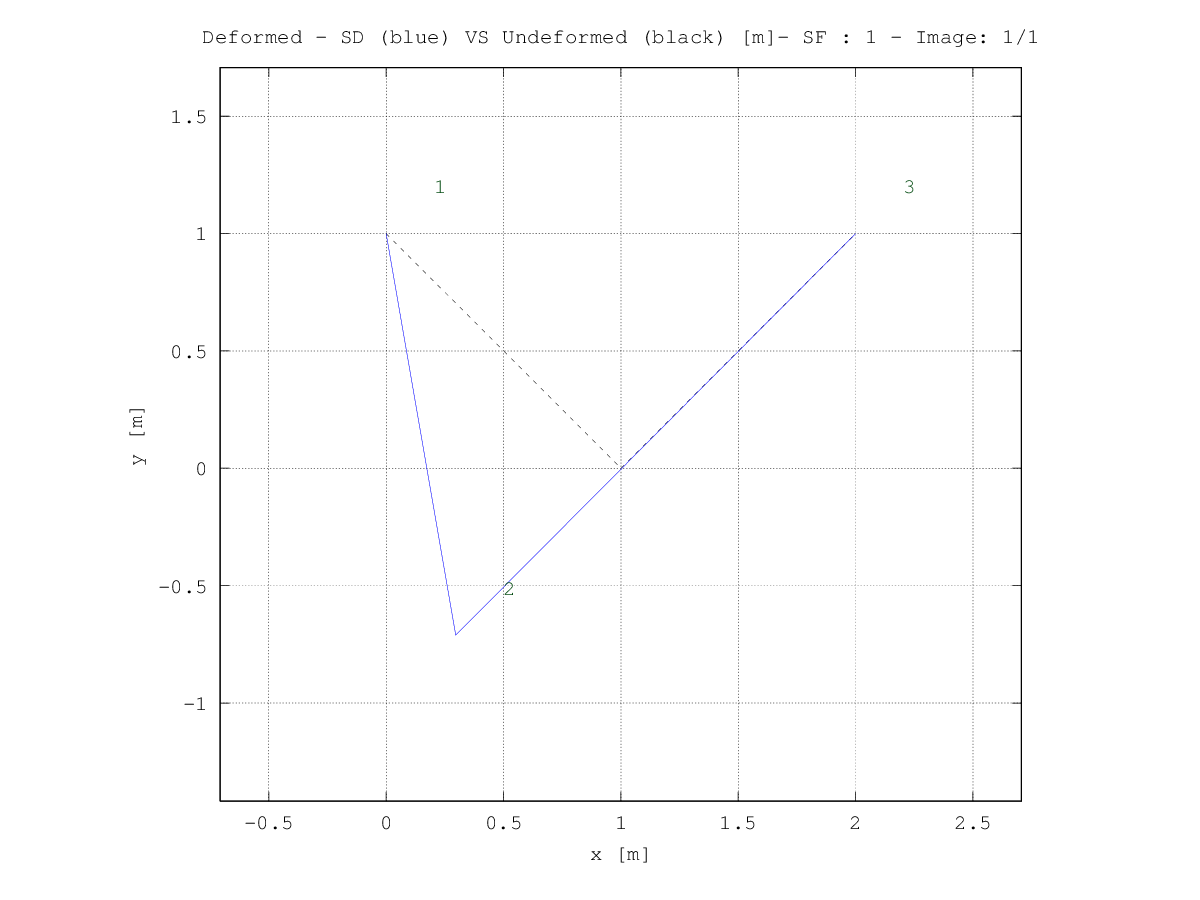
\includegraphics[width=.80\textwidth]{../../deformed/Prueba_deformed_1.png}      

\end{center}       
\newpage       

\section{Axial force}

\begin{center}                                   
\begin{longtable}{|R{1.5cm}|R{2.5cm}|}                      
\toprule[0.8mm]                                  
\multicolumn{2}{|c|}{Linear Axial Force} \\      
\midrule[0.5mm]                                  
Element   &   Force (kN)                  \\         
\midrule[0.5mm]                                  
\endfirsthead                                    
\toprule[0.8mm]                                  
\multicolumn{2}{|c|}{Linear Axial Force} \\      
\midrule[0.5mm]                                  
Element   &   Force (kN)                  \\         
\midrule[0.5mm]                                  
\endhead                                         
\hline                                           
\multicolumn{2}{r}{Next page...}                 
\endfoot                                         
\endlastfoot                                     
 {\color{OliveGreen}   1} & {\color{OliveGreen}        7.07 $\times 10^{          -1}}$ \\
 {\color{red}   2} & {\color{red}        7.07 $\times 10^{          -1}}$ \\
\bottomrule[0.8mm]                               
\caption{Linear Axial Force}             
\end{longtable}                                  
\end{center}                                     

\newpage       
\begin{center}       
Images for linear elasticity 

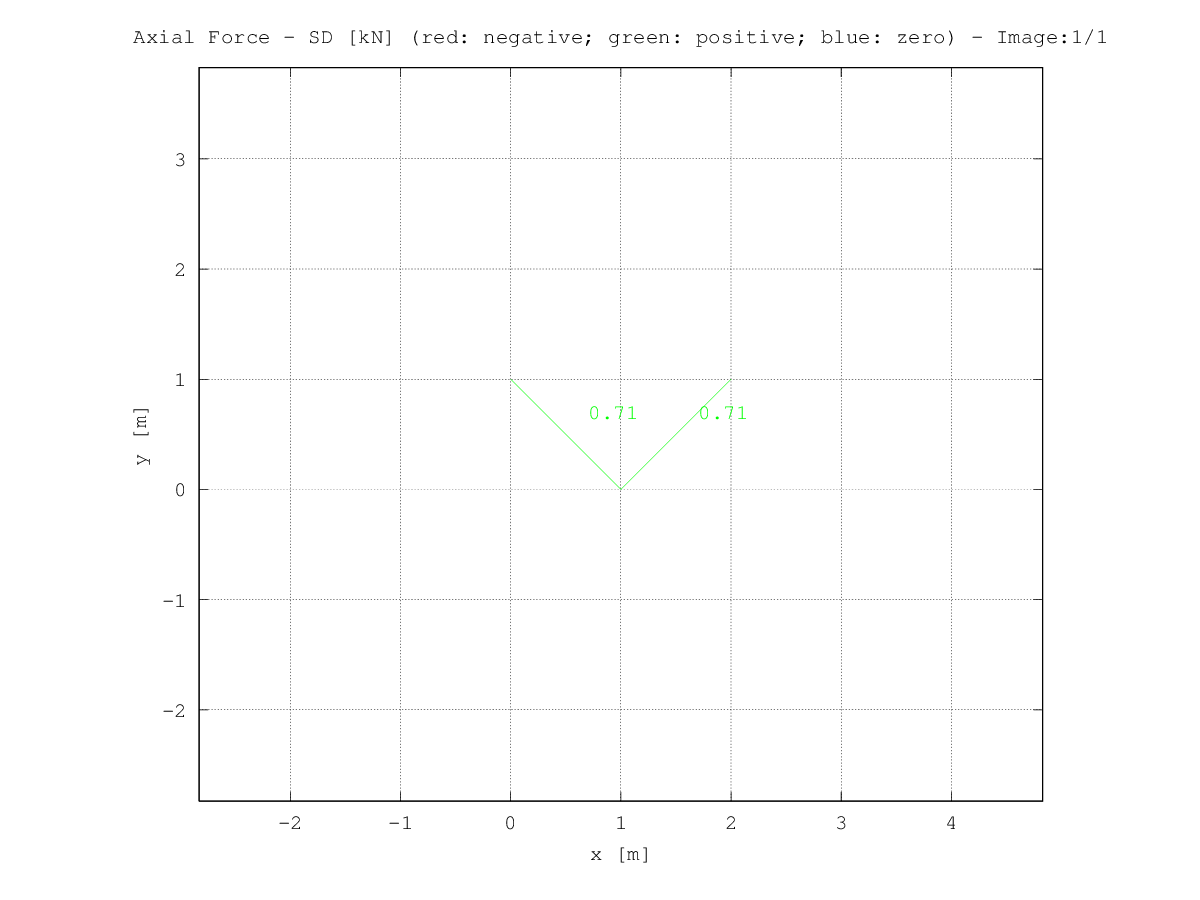
\includegraphics[width=.80\textwidth]{../../axial_force/Prueba_axial_force_1.png}      

\end{center}       
\newpage       

\section{Stresses}

\begin{center}                                   
\begin{longtable}{|R{1.5cm}|R{2.5cm}|}                      
\toprule[0.8mm]                                  
\multicolumn{2}{|c|}{Linear stress} \\      
\midrule[0.5mm]                                  
Element   &   Stress (kN/m$^\text{2}$)                  \\         
\midrule[0.5mm]                                  
\endfirsthead                                    
\toprule[0.8mm]                                  
\multicolumn{2}{|c|}{Linear stress} \\      
\midrule[0.5mm]                                  
Element   &   Stress (kN/m$^\text{2}$)                  \\         
\midrule[0.5mm]                                  
\endhead                                         
\hline                                           
\multicolumn{2}{r}{Next page...}                 
\endfoot                                         
\endlastfoot                                     
 {\color{red}   1} & {\color{red}        3.54 $\times 10^{          -3}$}\\
 {\color{OliveGreen}   2} & {\color{OliveGreen}        7.07 $\times 10^{          -1}$} \\
\bottomrule[0.8mm]                               
\caption{Linear Stress}             
\end{longtable}                                  
\end{center}                                     

\newpage       

\section{Strains}

\begin{center}                                   
\begin{longtable}{|R{1.5cm}|R{2.5cm}|}                      
\toprule[0.8mm]                                  
\multicolumn{2}{|c|}{Linear Strain} \\      
\midrule[0.5mm]                                  
Element   &   Strain                   \\         
\midrule[0.5mm]                                  
\endfirsthead                                    
\toprule[0.8mm]                                  
\multicolumn{2}{|c|}{Linear Strain} \\      
\midrule[0.5mm]                                  
Element   &   Strain                   \\         
\midrule[0.5mm]                                  
\endhead                                         
\hline                                           
\multicolumn{2}{r}{Next page...}                 
\endfoot                                         
\endlastfoot                                     
 {\color{red}   1} & {\color{red}        3.54 $\times 10^{          -3}$} \\
 {\color{OliveGreen}   2} & {\color{OliveGreen}        7.07 $\times 10^{          -1}$} \\
\bottomrule[0.8mm]                               
\caption{Linear Strain}             
\end{longtable}                                  
\end{center}                                     

\newpage  
\listoftables  
\end{document}  
